\documentclass[9pt,twocolumn,twoside]{pnas-new}
% Use the lineno option to display guide line numbers if required.

\templatetype{pnasresearcharticle} % Choose template
% {pnasresearcharticle} = Template for a two-column research article
% {pnasmathematics} %= Template for a one-column mathematics article
% {pnasinvited} %= Template for a PNAS invited submission

%% ABOVE THIS LINE IS PNAS TEMPLATE
%% BELOW THIS LINE IS MY STUFF

% \usepackage[utf8]{inputenc}
% \usepackage{amssymb}
% \usepackage{floatpag}
% \usepackage{bm}
% % \usepackage{algorithm2e}
% \usepackage{hyperref}
\usepackage[capitalise]{cleveref}
% \usepackage{csquotes}
% \usepackage[T1]{fontenc}
% \usepackage{textcomp} % provide symbols
% \usepackage{xr}
% \usepackage{afterpage}
% \usepackage{caption}
\usepackage{numprint}
\npfourdigitnosep
\npdecimalsign{.}
% % \usepackage{microtype}
% \usepackage{todonotes}

\newcommand\set{\mathcal}
\def\dist{\sim}
\DeclareMathOperator{\BB}{BetaBin}
\DeclareMathOperator{\GamDist}{Gamma}
\DeclareMathOperator{\N}{N}
\DeclareMathOperator{\logit}{logit}

% Macros for common abbreviations to get the spacing right
% See: https://stackoverflow.com/questions/3282319/correct-way-to-define-macros-etc-ie-in-latex
\usepackage{xspace}
\makeatletter
\DeclareRobustCommand\onedot{\futurelet\@let@token\@onedot}
\def\@onedot{\ifx\@let@token.\else.\null\fi\xspace}
\def\eg{e.g\onedot} \def\Eg{{E.g}\onedot}
\def\ie{i.e\onedot} \def\Ie{{I.e}\onedot}
\def\cf{c.f\onedot} \def\Cf{{C.f}\onedot}
\def\etc{etc\onedot} \def\vs{{vs}\onedot}
\def\wrt{w.r.t\onedot} \def\dof{d.o.f\onedot}
\def\etal{et al\onedot}
\makeatother
\begin{document}


\title{Using SARS-CoV-2 prevalence surveys for pandemic surveillance}

% Use letters for affiliations, numbers to show equal authorship (if applicable) and to indicate the corresponding author
\author[a]{Joshua Blake}
\author[]{TBC}
\author[b,a]{Paul Birrell}
\author[a,b]{Daniela De Angelis}

\affil[a]{MRC Biostatistics Unit}
\affil[b]{UKHSA}

% Please give the surname of the lead author for the running footer
\leadauthor{Blake}

% Please add a significance statement to explain the relevance of your work
\significancestatement{Understanding the transmission dynamics of SARS-CoV-2 is essential for guiding public health interventions. This study demonstrates the potential of data from prevalence surveys, specifically from the Coronavirus Infection Survey, to provide reliable estimates of viral incidence and transmission. This gold-standard survey selected individuals representative of the general population, unlike most sources of data from which transmission dynamics can be inferred. The findings highlight the importance of integrating large-scale, randomly sampled prevalence surveys into pandemic surveillance systems.}

% Please include corresponding author, author contribution and author declaration information
\authorcontributions{Please provide details of author contributions here.}
\authordeclaration{Please declare any competing interests here.}
\correspondingauthor{\textsuperscript{2}To whom correspondence should be addressed. E-mail: author.two\@email.com}

% At least three keywords are required at submission. Please provide three to five keywords, separated by the pipe symbol.
\keywords{Keyword 1 $|$ Keyword 2 $|$ Keyword 3 $|$ ...}

\begin{abstract}
During the pandemic caused by the SARS-CoV-2 virus, the UK’s Office for National Statistics ran a large prevalence survey, the Coronavirus Infection Survey (CIS).
Individuals enrolled in CIS were tested on a predetermined schedule, meaning the testing process was not biased by individuals' propensity to test and/or infectious status.
%removing  most reporting biases.
Here, we develop methods to investigate whether the CIS, designed to provide prevalence estimates, can be used to derive estimates of incidence and transmission.
To do so, we estimate incidence and transmission, fitting to only CIS data, using phenomenological and mechanistic models.
%taking two approaches: one phenomenological and one mechanistic.
These approaches are complementary, trading off bias and variance, and unravelling different aspects of the transmission dynamics.
We call for further work to optimise prevalence surveys as a leading tool for future pandemic surveillance.
\end{abstract}

\dates{This manuscript was compiled on \today}
\doi{\url{www.pnas.org/cgi/doi/10.1073/pnas.XXXXXXXXXX}}


\maketitle
\thispagestyle{firststyle}
\ifthenelse{\boolean{shortarticle}}{\ifthenelse{\boolean{singlecolumn}}{\abscontentformatted}{\abscontent}}{}

\firstpage{6}
% Use \firstpage to indicate which paragraph and line will start the second page and subsequent formatting. In this example, there are a total of 11 paragraphs on the first page, counting the first level heading as a paragraph. The value {12} represents the number of the paragraph starting the second page. If a paragraph runs over onto the second page, include a bracket with the paragraph line number starting the second page, followed by the paragraph number in curly brackets, e.g. "\firstpage[4]{11}".


% If your first paragraph (i.e. with the \dropcap) contains a list environment (quote, quotation, theorem, definition, enumerate, itemize...), the line after the list may have some extra indentation. If this is the case, add \parshape=0 to the end of the list environment.
\dropcap{T}he pandemic caused by the SARS-CoV-2 has resulted in a horrific toll on humanity, inflicting 31 million deaths~\citep{whoCOVIDExcess,economistCOVIDExcess}, stretching healthcare services to the brink of collapse~\citep{fongNHS}, and disrupting societies worldwide.
The impact motivated governments to invest in infectious disease surveillance on a scale never previously seen.

An example of such a system in the UK's Office for National Statistics (ONS)'s Coronavirus Infection Survey (CIS)~\citep{cisMethodsONS,CIS}.
CIS was a gold-standard survey, inviting households selected at random from the population to partake and testing individuals in them on a regular schedule, minimizing biases associated with voluntary testing.
CIS required a level of resources rarely available to infectious disease surveillance systems but provided SARS-CoV-2 surveillance without relying on individuals' ability or desire to test and independent of the severity of their disease.
Data without these issues, which makes the data unrepresentative of the population, was rarely available in the pandemic~\citep{shadboltChallenges}.
CIS was primarily designed to allow weekly estimates of prevalence (which we define as the proportion of the population testing positive for SARS-CoV-2 using a Reverse Transcription Polymerase Chain Reaction (RT-PCR) test at a given time), stratified by age and region, and adjusting for the non-representativeness caused by different response rates among different demographic groups; these estimates were published weekly by ONS~\citep{pouwelsCommunity,pouwelsMRPvaccination,cisMethodsONS,onsCISdec2020}.

However, prevalence is a delayed indicator and does not relate directly to the time that the infections occur; the latter is important for understanding how transmission has changed in response to control measures and other interventions.
Instead, incidence, the number of new infections over a specific period, is a more useful metric but requires statistical measures to estimate as it can almost never be directly observed.
Furthermore, some statistical methods allow the direct inference of how a virus is being transmitted providing even richer information for informing the response.
A variety of methods can be used to estimate incidence and transmission, with methods often categorized by how explicitly they represent the underlying biological and epidemiological processes.

At one extreme, phenomenological (sometimes known as ``statistical'') models make minimal assumptions about the underlying processes, instead flexibly describing the trends in the data~\citep{beckerCOVIDmodels}.
This approach helps reduce potential biases but cannot capture the underlying dynamics of transmission.

At the other extreme, fully mechanistic models explicitly represent the mechanism that generates new infections the state of each individual in the population and the processes that drive the spread of the virus~\citep{andersonInfectious,keelingModeling}.
This type of models provide deeper insights into transmission dynamics, such as the rate at which the virus spreads and the susceptibility of different demographic groups.
In this work, we develop both phenomenological and mechanistic models to analyse the CIS data.

During the pandemic, various methods were proposed to estimate incidence and transmission from CIS data. However, these methods often combined CIS data with other data sources, oversimplified the duration of PCR positivity, or did not fully account for the uncertainty in the survey data. Our study advances these efforts by fitting models solely to CIS data, providing a more accurate representation of the duration of PCR positivity and improving the quantification of survey uncertainty.

CIS's comprehensive and consistently collected data offer a unique opportunity to derive critical epidemiological metrics without relying on additional data sources.
In this proof-of-concept study, we show that CIS, designed primarily to measure prevalence, can also be the basis of incidence and transmission estimation, and provide guidance on appropriate methodologies for this purpose.
By fitting both phenomenological and mechanistic models to CIS data, we demonstrate the feasibility and robustness of these approaches. 

The phenomenological model provides a flexible framework with minimal assumptions, while the mechanistic model offers detailed insights into transmission dynamics.

In this paper, we present the results of our analysis, highlighting the strengths and limitations of each modelling approach. We show that CIS data can be used not only to estimate prevalence but also to derive accurate estimates of incidence and transmission. These findings underscore the potential of prevalence surveys like CIS to serve as a cornerstone for pandemic surveillance and response.

Our study emphasizes the importance of optimizing the design and implementation of future prevalence surveys to enhance their utility in monitoring and controlling pandemics. By leveraging high-quality, large-scale data from surveys like CIS, public health authorities can make more informed decisions and implement more effective interventions to mitigate the impact of infectious diseases.

\section*{Results}

We fit two models to the X positive and Y negative tests between DATES in England.

The first model, a phenomenological model, was fit to the test results stratified by region, sex, age group, and ethnicity using a methodology based on dynamic multi-level regression and poststratification (MRP), a Bayesian methodology for accounting for non-response bias in a flexible framework.
It does not represent any aspect of the disease or population within the model, allowing a computationally-efficient inference methodology, the integrated Laplace approximation (INLA), to be used, required to incorporate the many parameters needed to stratify the data more granularly.
This leads to a more flexible model which can capture arbitrary trends in prevalence in different groups while penalising over-fitting; furthermore, it more comprehensively captures issues with non-response.

The second model, a mechanistic model, is a SEIR model, meaning it tracks the proportion of population that are Susceptible, Exposed (infected but not yet infectious), Infectious, and Removed (\ie no longer infectious but playing no further part in the pandemic because they are immune or dead).
The model stratifies these groups by region and age which partially accounts for the non-response and more accurately captures the pandemic's dynamics.
Susceptible individuals can become exposed by their interaction with infectious individuals, through contact rates stratified by age.
These rates combine by pre-pandemic surveys with real-time data on time-use.
By representing these proportions and their interactions, we can estimate more detail over the transmission process; however, the stronger assumptions required could introduce bias into the estimation.

We estimated incidence proportion, the proportion of the population (or a subpopulation) newly infected on each day~\citep{lashModern}.

\subsection*{Incidence estimates}

Both models successfully produce estimates of SARS-CoV-2 incidence proportion, the proportion of the population that becomes PCR positive on a given day (\cref{fig:incidence}(A)).
The results largely agree with each other and previous knowledge (REF), demonstrating the robustness of the data and approaches.
They show a slow rise and plateau in autumn, a decrease during November, then a fast increase peaking near the end of 2020.
The mechanistic model produces tighter credible intervals, reflecting the additional information it uses about the underlying transmission dynamics.
\begin{figure*}%[tbhp]
\centering
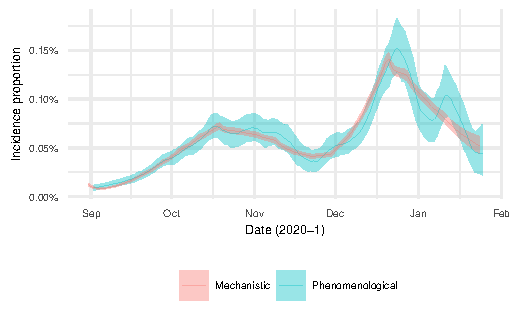
\includegraphics{figures/incidence}
\caption{%
    Incidence estimates (median and 95\% credible interval) from both models.
    Incidence proportion is the proportion of the population that becomes PCR positive on a given day.
    (A) Estimates for the whole of England.
    (B) Estimates by age group for the North East region.
    Remaining regions shown in TODO: add other regions to appendix.
}
\label{fig:incidence}
\end{figure*}

The largest disagreement between the models is that the phenomenological model estimates a second peak in incidence in January, although the credible intervals overlap for the majority of the period.

\subsection*{Impact of model assumptions}

Age-specific results for the North East region clearly show the impact of model assumptions on the estimates (\cref{fig:incidence}(B)).
The 12--16 age group decreases in incidence significantly during the school half-term break which is directly introduced into the model through modification of the number of contacts which school age children have, informed by school attendance data (see Methods and Materials).

Disagreement between the two models in the 12--16 and 17--25 age groups are also prominent.
The mechanistic model has a more rigid structure (fewer parameters) limiting its ability to capture all changes in incidence, especially when changes in transmission differ between age groups.
Therefore, when fitting, it appears to compromise these two age groups in opposite directions: overestimating the prevalence and incidence in the 12--16 age group and underestimating it in the 17--25 age group (TODO: ref a supplementary figure with goodness-of-fit).

The phenomenological model is more flexible and therefore has a better fit to the data in these age groups.
It is fit to more granular groupings of individuals, improving the adjustment for non-response bias, but this means that for privacy reasons we cannot show the fit.

\subsection*{Decomposition of transmission components}

A major advantage of using a mechanistic model is the ability to decompose the components of transmission.
The mechanistic model decomposes changing transmission into three components: changes in contact patterns, measured through Google Mobility data; changes in levels of susceptibility in the population; and a remaining unexplained component, which includes behavioural changes such as masking or improved case-finding leading to a higher proportion of infectious individuals being isolated and biological changes (\eg variants).
The unexplained component is often of interest to policy-makers because reducing transmission with minimal effects on contacts (which often have larger economic or social benefits) is a common policy goal.

We estimate that this component initially decreases over the period studied (from September 2020), is flat for a few weeks, then rises in November and December (\cref{fig:rw} and TODO other regions in supplement).
The increase in the unexplained component in November and December is correlated with the rise of the Alpha variant.
\begin{figure}%[tbhp]
\centering
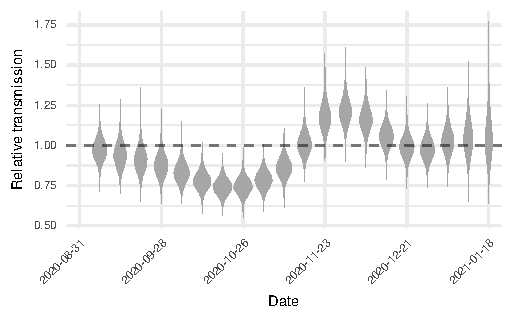
\includegraphics{figures/rw}
\caption{%
    The component of transmission not explained by changes in contact patterns (as measured by Google Mobility data) and increasing population immunity.
    Shown is a violin plot of the posterior distribution.
    London shown, for other regions see TODO: add other regions to appendix.
}
\label{fig:rw}
\end{figure}

\subsection*{Difference in transmission by age}

An advantage of the CIS dataset is that it captures all age groups over two years old in a well-understood way.
The mechanistic model can exploit this data to estimate how susceptibility differs by age.
Here, susceptibility is defined as the probability of a susceptible individual becoming infected upon contact with an infectious individual which includes both biological factors (\eg differences in immune response) and behavioural factors (\eg differences in hygiene).
We estimate this parameter independently for each region, showing that children are less susceptible by around 20\% than adults in all regions (\cref{fig:children}).
\begin{figure}%[tbhp]
\centering
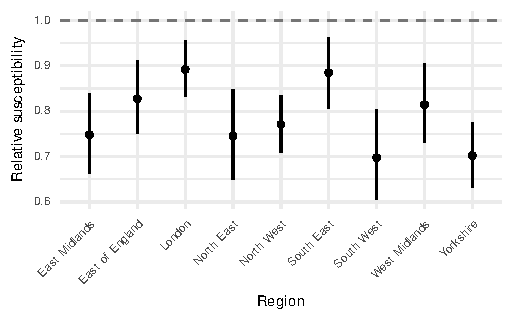
\includegraphics{figures/children}
\caption{%
    How susceptible (likely to be infected upon contact with an infectious individual) children are relative to adults.
    Estimate is per region (posterior median and 95\% credible interval shown). 
}
\label{fig:children}
\end{figure}

\section*{Discussion}

We have demonstrated that a range of important epidemiological estimates can be derived from prevalence survey data, specifically using the Coronavirus Infection Survey.
Our study utilized two distinct models---a phenomenological model and a mechanistic transmission model---both of which were successfully fit to CIS data.

Using a single, well-designed study like CIS as a data source leads to robust and reliable estimates.
CIS's biases, primarily due to non-response, are well understood and can be accounted for in the models.
This is unlike other data sources, such as testing data, where how many tests and who is tested can change over time for measured (\eg testing capacity) and unmeasured reasons (\eg public perception of risk).

Furthermore, the high retention rates of CIS following recruitment mean that any bias is consistent over time; therefore, the inference of trends from this data is particularly robust.
Trends, such as how quickly the epidemic is growing, are often more important than absolute levels.
Otherwise reliable data sources, such as the number of patients hospitalized with SARS-CoV-2 infections, can be affected by factors such as admission policies and bed availability (REF).
These data sources primarily reflected incidence in elderly and other vulnerable groups (REF), whereas CIS captures all age groups over two years old.
The implication for transmission in young adults and children must then be based on model assumptions or indirect evidence, such as contact surveys or mobility data (REF).
Here, we exploit this to estimate how susceptibility differs by age, showing that children are less susceptible than adults.

To overcome the limitations of any specific data sources, many previous studies of SARS-CoV-2 in England (REF) have utilized evidence synthesis techniques (REF).
These techniques combine multiple data sources, such as testing data, hospitalizations, and deaths, to estimate the underlying transmission dynamics.
However, these methods are complex and require assumptions regarding how the data sources are related.
If different data sources conflict, then this should be resolved manually which is time-consuming and often subjective.
By using a single data source, we avoid these issues and provide a more direct inference of the underlying transmission dynamics.
Furthermore, the use of a single data source means that inferences can more directly be linked to the data source aiding debugging and interpretation of model outputs.

Our study reinforces the value of using different models with different assumptions to estimate the same quantity.
The mechanistic model often provides more useful insights, by decomposing the components of transmission, estimating how susceptibility differs by age, and producing narrower credible intervals.
However, the phenomenological model is more flexible and can better fit the data, particularly in granular subpopulations.
Furthermore, it includes ethnicity as a covariate, which can help provide an equitable response to the pandemic and better adjusts for the non-response bias in the survey.
Extending mechanistic models to include ethnicity should be considered as a priority for future work, which would require contact surveys in ethnic minority populations.

Comparing the results can highlight modelling issues; in our case, the mechanistic model's inability to capture changes in transmission among age groups.
A more flexible model could be developed to capture these changes; however, current work is limited by the computational burden of fitting mechanistic models to large datasets.
Further work could extend approximate Bayesian methods, such as the integrated Laplace approximation used in the phenomenological model, to mechanistic models.
As well as allowing for more flexible models, capturing age-specific changes over time, such work would allow faster model fitting, a high-priority when responding to an emergency such as a pandemic.

Our analysis has important implications for future pandemic preparedness and response.
We have shown that a prevalence survey with randomly-selected participants are extremely useful for monitoring an ongoing pandemic.
Yet these gold-standard surveys were conducted by few countries during the SARS-CoV-2 pandemic.
A major barrier is that they are expensive.
Further work should explore how to reduce the cost of these surveys, for example by using cheaper testing methods or studying more carefully the impact of alternative study designs allowing the same information to be inferred using fewer participants.
This could involve varying the testing schedule or the selection criteria.
Finally, we call for such studies to be embedded into pandemic plans for sufficiently severe pandemics.

\matmethods{

\subsection*{CIS study design and data}
The CIS~\citep{CIS} was set up in April 2020 as a large-sclae, longitudinal scale study across the pandemic.
Individuals were originally recruited in England from those who had previously responded to ONS survey(s); it was expanded in September 2020 using a random sample of addresses across the whole UK.
Following enrolment and consent, individuals were visited on a pre-determined schedule.
At each visit, a questionnaire was completed and a combined throat and nose swab was collected for RT-PCR testing, along with various other pieces of data.
We consider only the result of the RT-PCR testing.
Enrolment was continuously ongoing until 31st Jan 2022, with data collected until 13th Mar 2023~\citep{weiRisk}. 

We use all negative and positive tests (\ie discarding void test results) in England between Mon 31 Aug 2020 and Sun 24 Jan 2021 for this proof-of-concept study.
During this period, the CIS was of sufficient size, and transmission was sufficiently high, to provide enough data for the analyses.
Second, incidence began to rise over this period, after the fall due to the first lockdown.
Additionally, this period ends before substantial vaccine roll-out, which affected many important aspects of the analysis; most relevantly, the duration of detectability and the susceptibility of the population.

We grouped tests by region and age for both analyses.
In the phenomenological model, we also grouped tests by sex and ethnicity, due to there being evidence of differential non-response in these groups~\citep{pouwelsCommunity}.
However, the additional stratification is not possible in the mechanistic model due to computational constraints and a lack of contact data for these groups.
For regions, we used the nine regions of England (International Territorial Level 1); these are: North East, North West, Yorkshire and the Humber (commonly abbreviated to Yorkshire), East Midlands, West Midlands, East, London, South East, and South West~\citep{onsRegions}.
For age groups, we used under 11 (pre-school and primary school), 12--16 (compulsory secondary school), 17--25 (adolescents and young adults who may remain in formal education), 26--50 (younger working age adults), 51--70 (older working age adults), and 71+ (elderly).
We used two levels of ethnic grouping.
Broad groupings (White and non-White), because the White population makes up over 80\% of the UK, and more granular groupings (Asian, Black, Mixed, White, and Other).


\subsection*{Phenomenological model}
The phenomenological model consists of three steps.
First, a Bayesian multi-level logistic regression model is fit to the data to estimate the probability of a positive test for a variety of population strata (described below) on each day considered.
Next, deconvolution (described below) is used to calculate the incidence proportion in each stratum on each day implied by the probability of a positive test for each of 500 samples from the approximate posterior of the regression model.
Finally, the incidence proportions are poststratified to the population and subpopulations of interest to estimate the incidence proportion in each subpopulation on each day.
The full algorithm for this procedure is given in the SI Methods.

\subsection*{Regression model}
We modify a previously-used regression model~\citep{pouwelsMRPvaccination} for the same dataset to be suitable for estimating incidence.
The model is fit independently to each region in a Bayesian framework using the Integrated Nested Approximation (INLA, implemented in R-INLA)~\citep{RINLA,rueINLA}.
Each day, the probability of a positive test for a given age group, ethnicity, and sex is modelled as a logistic regression with fixed effects for sex and White or non-White ethnicity; and random effects for age group, including its interaction with time, and time.
To account for the overdispersion due to the household-based design of the survey and unobserved heterogeneity, we use a beta-binomial likelihood.
See SI Methods for further details.

\subsection*{Deconvolution}

Deconvolution for estimating incidence from prevalence was popularized in infectious disease epidemiology by the backcalculation method for HIV/AIDS incidence estimation~\citep{brookmeyerBackcalculation}.
In this context, it means that the incidence proportions for stratum $i$ on day $t$, $Z_{t,i}$ can be calculated sequentially for $t = 1, \dots, T$ from the prevalence on days $1, \dots, t$ in that stratum, $P_{1,i}, \dots, P_{t,i}$ using the forward-substitution method~\citep{cormenMatrix}:
\begin{equation}
    Z_{t,i} = P_{t,i} - \sum_{s=1}^{t-1} Z_{s,i} S(t-s+1)
\end{equation}
where $S(t-s+1)$ is the probability of a positive test on day $t-s+1$ given that the individual was infected on day $s$.
Further details are provided in SI Methods.

\subsection*{Poststratification}
Poststratification aggregates the incidence proportions in different stratum to be representative of a (sub)population, here England or one of its regions.
Specifically, define a (sub)population of interest as a set of strata $\set{S}$.
Then the incidence proportion in the (sub)population on day $t$ is
\begin{align}
Z_t(\set{S})
&= \frac{\sum_{j \in \set{S}} Z_{j,t} N_j}{\sum_{j \in \set{S}} N_j}
\label{backcalc:eq:poststratify}
\end{align}
where $N_j$ is the population size of stratum $j$, provided by the ONS.

\subsection*{Mechanistic model}
The mechanistic model is a deterministic, compartmental SEIR model, including age-structure.
This means that the state of the population is represented by the proportion of individuals of each age in each of four compartments: susceptible (S), exposed (E), infectious (I), and recovered (R).
The model then evolves according to a set of ordinary differential equations (ODEs).
The SEIR model is a standard model~\citep{andersonInfectious,keelingModeling}, which we make two adjustments to: allowing the transmission rates between age groups to vary over time and adding an observation model to relate the model to CIS data.
The starting state and parameters of the ODEs are inferred in a Bayesian framework.

\subsection*{Transmission rates}
The rate of transmission between infectious and susceptible individuals in the model is based on three components: the number of contacts between individuals, the probability of transmission given a contact, and the proportion of the population that is susceptible.
The number of contacts between different age groups were based on POLYMOD~\citep{mossongSocial} and adjusted on a weekly basis using Google Mobility data~\citep{googleCOVID19} according to a previously described method~\citep{vanleeuwenAugmenting,birrellRealtime}.
The probability of transmission given a contact is assumed to be constant across age groups except that children and adults are allowed to have different susceptibilities, as described by previous work~\citep{vinerTransmission}; however, the probability is allowed to vary each week to capture the impact of changes not present elsewhere in the model (see SI Methods for details).
The proportion of the population that is susceptible is part of the system of ODEs.

\subsection*{Observation model}
The observation model relates the transmission process in the mechanistic model, just described, to the data.
A set of states approximates the length of time an individual is positive for SARS-CoV-2 following infection; we use a more accurate approximation of this time than much previous work.
These states are then used to calculate the probability of a positive test on each day for each stratum.
Finally, the probability of a positive test is used to calculate the likelihood of the data, the number of positive tests on each day in each stratum.
A full description of the observation model is provided in SI Methods.

\subsection*{Inference}
We fit the mechanistic model in a Bayesian framework using Markov chain Monte Carlo (MCMC)~\citep{hastingsMCMC,gelmanBDA}.
Informative priors were used for the starting state of the model and the rates of progression through the model; this is required for identifiability~\citep{dankwaStructural}.
We used weakly informative priors for all other parameters (TODO ref table with priors).
Bespoke Markov chain Monte Carlo code, adapted from a previous study~\citep{ghoshApproximate}, was used to estimate the posterior distribution of the parameters of the mechanistic model.
Proposals were drawn from a multivariate normal distribution, adapted throughout the inference process~\citep{andrieuTutorial} and accepted or rejected based on the Metropolis--Hastings algorithm~\citep{hastingsMCMC}.
All results are based on four Markov chains each of length \numprint{1000000} iterations for each region.
The first \numprint{500000} were discarded as burn-in, with the remaining chains thinned to every \numprint{100}th iteration.
This gives \numprint{5000} posterior samples per region.
This was further thinned to \numprint{2000} samples when calculating posterior predictive quantities (incidence and prevalence) due to their computational cost.
}

\showmatmethods{} % Display the Materials and Methods section

\acknow{Please include your acknowledgments here, set in a single paragraph. Please do not include any acknowledgments in the Supporting Information, or anywhere else in the manuscript.}

\showacknow{} % Display the acknowledgments section


\bibsplit[15]
%Use \bibsplit to split the references from the body of the text. Value "[2]" represents the number of reference in the left column (Note: Please avoid single column figures & tables on this page.)

% Bibliography
\bibliography{references}

\clearpage
\appendix

\section*{Supplementary methods: phenomenological model}

TODO: insert full algorithm for method, \ie how the different pieces described below and in the main text are composed.

\subsection*{Logistic regression model}

We use a modified version of a previous Bayesian multi-level logistic regression model for the CIS~\citep{pouwelsMRPvaccination}.
A regression model serves two purposes: first, it allows borrowing of information between days and stratum; second, it corrects for non-response bias.

For a day $t$, age group $a$, ethnicity $e$, and sex $s$ the regression model is:
\begin{align}
    \logit(p_{taes}) &= \beta + \beta_s + \beta_{w(e)} + u_a + v_e + w_t + l_{a,t} \\
    y_{taes} &\dist \BB(n_{taes}, p_{taes}, \rho).
\end{align}
The terms are as follows.
\begin{itemize}
    \item $n_{taes}$ and $y_{taes}$ are the number of individuals tested and the number of positive test results respectively on day $t$ in individuals of age group $a$, ethnicity $e$, and sex $s$. We use a beta-binomial distribution for the likelihood. A beta-binomial distribution is an overdispersed version of the binomial distribution~\citep{hughesUsing}. Overdispersion allows for household clustering and other overdispersion in the data, which is common in epidemiological data~\citep{griffithsBBD}.
    \item $\beta$ is a global intercept term with the vague prior $\beta \dist \N(0, 1/0.001^2)$.
    \item $\beta_s$ is a fixed effect for sex, with $\beta_s = 0$ for males and estimated for females. The prior for $\beta_s$ is vague, $\beta_s \dist \N(0, 1/0.001^2)$.
    \item $\beta_{w(e)}$ is a fixed effect for White or non-White ethnicity. $\beta_{w(e)} = 0$ if $e$ corresponds to White ethnicity and $\beta_{w(e)} = \beta_{n}$ otherwise (\ie non-White ethnic groups).
      The prior for $\beta_n$ is vague, $\beta_n \dist \N(0, 1/0.001^2)$.
      % $\beta_n$ and $\beta_f$ have the default INLA prior for fixed effects\todo{check what this is}.
    \item $u_a$ and $v_e$ are independent normal random effects for age and ethnic group respectively. Their standard deviation has a penalized complexity prior~\citep{simpsonPenalising} with a 10\% probability of being greater than 1.
    \item $w_t$ is a second-order random walk, that is $w_t = 2w_{t-1} - w_{t-2} + \epsilon_t$ where $\epsilon_t \dist \N(0, \sigma_w^2)$.
      $\sigma_w$ has a vague prior, $1/\sigma_w \dist \GamDist(1, 5 \times 10^{-5})$.
    \item $l_{a,t}$ is an age-group specific second-order random walk.
      That is $l_{a,t} = 2l_{a,t-1} - l_{a,t-2} + \epsilon_{a,t}$ where $\epsilon_{a,t} \dist \N(0, \sigma_l^2)$.
      $\sigma_l$ has a vague prior, $1/\sigma_l \dist \GamDist(1, 5 \times 10^{-5})$.
\end{itemize}
The second-order random walk priors favours linear growth in $\logit(p_{taes})$ over time.
For the small values of $p_{taes}$ likely to be encountered, this approximates exponential growth.

\subsection*{Deconvolution}

TODO: incorporate relevant parts of thesis section 7.1.3.

The relationship between incidence and prevalence is stochastic; however, here a deterministic relationship is assumed.
This is a good approximation as long as the proportion of the population sampled by prevalence survey is small because the stochastic noise in the sampling process is much greater than that in the relationship between incidence and prevalence~\citep{blakeThesis}.

\section*{Supplementary methods: mechanistic model}

TODO: insert ODEs and other details of SEIR model.

\end{document}
